\chapter{Estado del Arte}

En este capítulo hablaremos, principalmente, de dos importantes aspectos. El primero es la situación de la industria del entretenimiento digital hoy en día, seguido de una definición sobre lo que es un \textit{roguelike}. El segundo son los elementos que dificultan y facilitan el uso de diferentes programas y \textit{software} a ciertos sectores de la sociedad como invidentes o daltónicos; cómo algunos programas intentan solventar estos problemas y las razones por las que hemos elegido introducir ciertos elementos en nuestro proyecto para diliar con los mismos.

\section{La industria del entretenimiento digital en la actualidad}

Desde sus primeros pasos hasta hoy en día, tal y como sucede con muchas de las novedades en el mundo del entretenimiento y la cultura, el sector del ocio digital ha sufrido cierto estigma por una gran parte de la población, siendo censurado y degragado en mayor o menor medida, no tan solo por cierta parte de la sociedad, pero también por muchos medios de comunicación y gobiernos. A pesar de que hoy en día este problema todavía está activo\footnote{Es común que cada año en Australia se censuren algunos juegos como \href{http://goo.gl/hFrQah}{Paranautical Activity} por razones que otras formas de entretenimiento y cultura como películas o libros no se ven tan afectados.}, la industria se ha expandido tanto (consolas, ordenadores, navegadores, Facebook, móvil...), que cada vez es más complicado encontrar a alguien que no haya jugado a algún videojuego en las últimas semanas, ya es algo que forma parte del día a día de mucha parte de la población.

\subsection{La industria, en números}
En todo el mundo, pero especialmente en EEUU, la industria de los videojuegos es uno de los sectores con más crecimiento \cite{website:gamesimprovingeconomy} llegando a generar, solamente en ventas digitales, alrededor de 61 billones de dólares en el año 2015 \cite{website:gamingsales}.

Este gran éxito se debe, en gran parte, a la irrupción de los juegos desarrollados para móviles, cuyo beneficio ha ido aumentando enormemente durante los últimos años. \footnote{\href{http://goo.gl/Lz9UAa}{La venta de videojuegos en Alemania crece año tras año, pero el mayor aumento de beneficio se está centrando en el mercado de los juegos para móvil}}. Sin embargo, esto no significa que el resto de plataformas no estén triunfando. Solamente Steam, la plataforma de distribución digital para PC por excelencia desarrollada por Valve, ha generado alrededor de 3 billones y medio de dólares en el año 2015\cite{website:steamgamesmarket}.

Con el mercado del PC resurgiendo, las consolas de sobremesa obteniendo grandes números de ventas, las portátiles resistiendo, el mercado de los videojuegos para móvil en esplendor y los cascos de realidad virtual llegando al mercado este año 2016; todo parece indicar que estos números no harán más que crecer durante los próximos años.

\subsection{Conclusión}

Lo que comenzó hace varias décadas como un modo de entretenimiento sin ninguna pretensión, generalmente enfocado a un público infantil o adolescente y que miraba a otras industrias como la cinematográfica con recelo, se ha convertido en todo lo que había deseado y más. Gracias a grandes títulos y a su expansión a toda clase de dispositivos, no se puede hablar de la industria del entretenimiento sin hablar de videojuegos y, en muchos casos, algunos de esos títulos han logrado ser nombrados como obras de arte en su género, pasando a la historia y siendo recordados a lo largo de los años.

\section{\textit{Roguelikes.}}
\label{sec:roguelikeinformacion}

\subsection{Qué es y orígenes}

En 1983, Michael Toy y Glenn Wichman crearon un videojuego llamado Rogue\footnote{Desde 2014 este juego se encuentra disponible en \href{https://archive.org/details/msdos_Rogue_1983}{archive.org}} que acabó definiendo un género.

Las características principales que definieron a Rogue y que, por extensión, definieron al género de los \textit{roguelikes} inicialmente, son:

\paragraph{Dificultad}: Rogue es un videojuego difícil con \textit{permadeath}\footnote{Una vez que el jugador muere, tiene que empezar desde el principio; no hay partidas guardadas} que obligará al jugador a rejugarlo una y otra vez, intentando llegar más lejos que la anterior partida gracias a ir aprendiendo los funcionamientos del mismo.

\paragraph{Aleatoriedad}: Cada vez que el jugador comienza una partida nueva se encontrará con ciertos elementos que han cambiado con respecto a la vez anterior: el mapa es distinto, los elementos y enemigos se encuentran en sitios diferentes, los objetos obtenidos han cambiado... causando que cada vez que el usuario empiece, tenga un grado de dificultad pseudo-aleatorio dependiendo de la semilla con la que estos elementos han sido generados.

\paragraph{Progresión}: Una de las frases más escuchadas en las críticas que Rogue recibió tras su lanzamiento es que el jugador sentía la necesidad de intentar llegar más lejos en cada ocasión\cite{website:machinesnetworks}. Esto viene dado, sobre todo, por la sensación de progresión y de que en cada \textit{run}\footnote{Palabra comúnmente usada en estos géneros y que se refiere a una partida desde su inicio hasta que el jugador pierde} el usuario vaya mejorando. Dentro de la propia partida también existe una progresión a medida que el usuario derrota enemigos, consiguiendo puntos de experiencia, subiendo niveles y obteniendo mejores armas y armaduras con las que ser un poco más fuerte.

\begin{figure}[h!]
		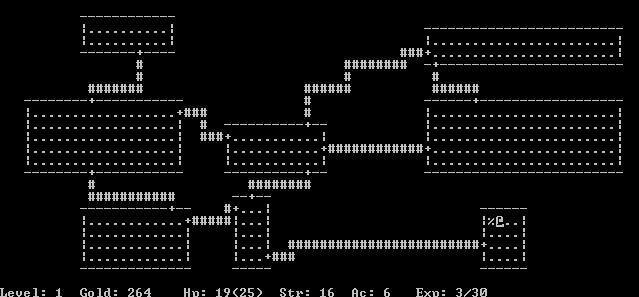
\includegraphics[width=\textwidth,height=\textheight,keepaspectratio]{./img/roguegame.PNG}
	\caption{Captura de pantalla de \href{https://en.wikipedia.org/wiki/File:Rogue_Unix_Screenshot_CAR.PNG}{dominio público} (tal y como todas las imágenes mostradas en este proyecto) del videojuego Rogue}
	\label{fig:roguegame}
\end{figure}

A partir de este momento muchos fueron los juegos que decidieron imitar estas características de Rogue, añadiendo, cambiando o enfatizando diferentes elementos, por eso se han denominado \textit{roguelikes}.

\subsection{En la actualidad}

Tras el éxito de Rogue, fueron muchos los títulos que simularon su fórmula de éxito e intentaron mejorarlo, sobre todo gráficamente. Algunos de ellos se centran en diferentes aspectos (combate en vez de exploración, por ejemplo) y llegan a ser completamente diferentes a la hora de jugarlos (por turnos o tiempo real) pero, sin embargo, todos conservan buena parte de las características que hicieron al género famoso hasta hoy en día.

\begin{figure}[h!]
		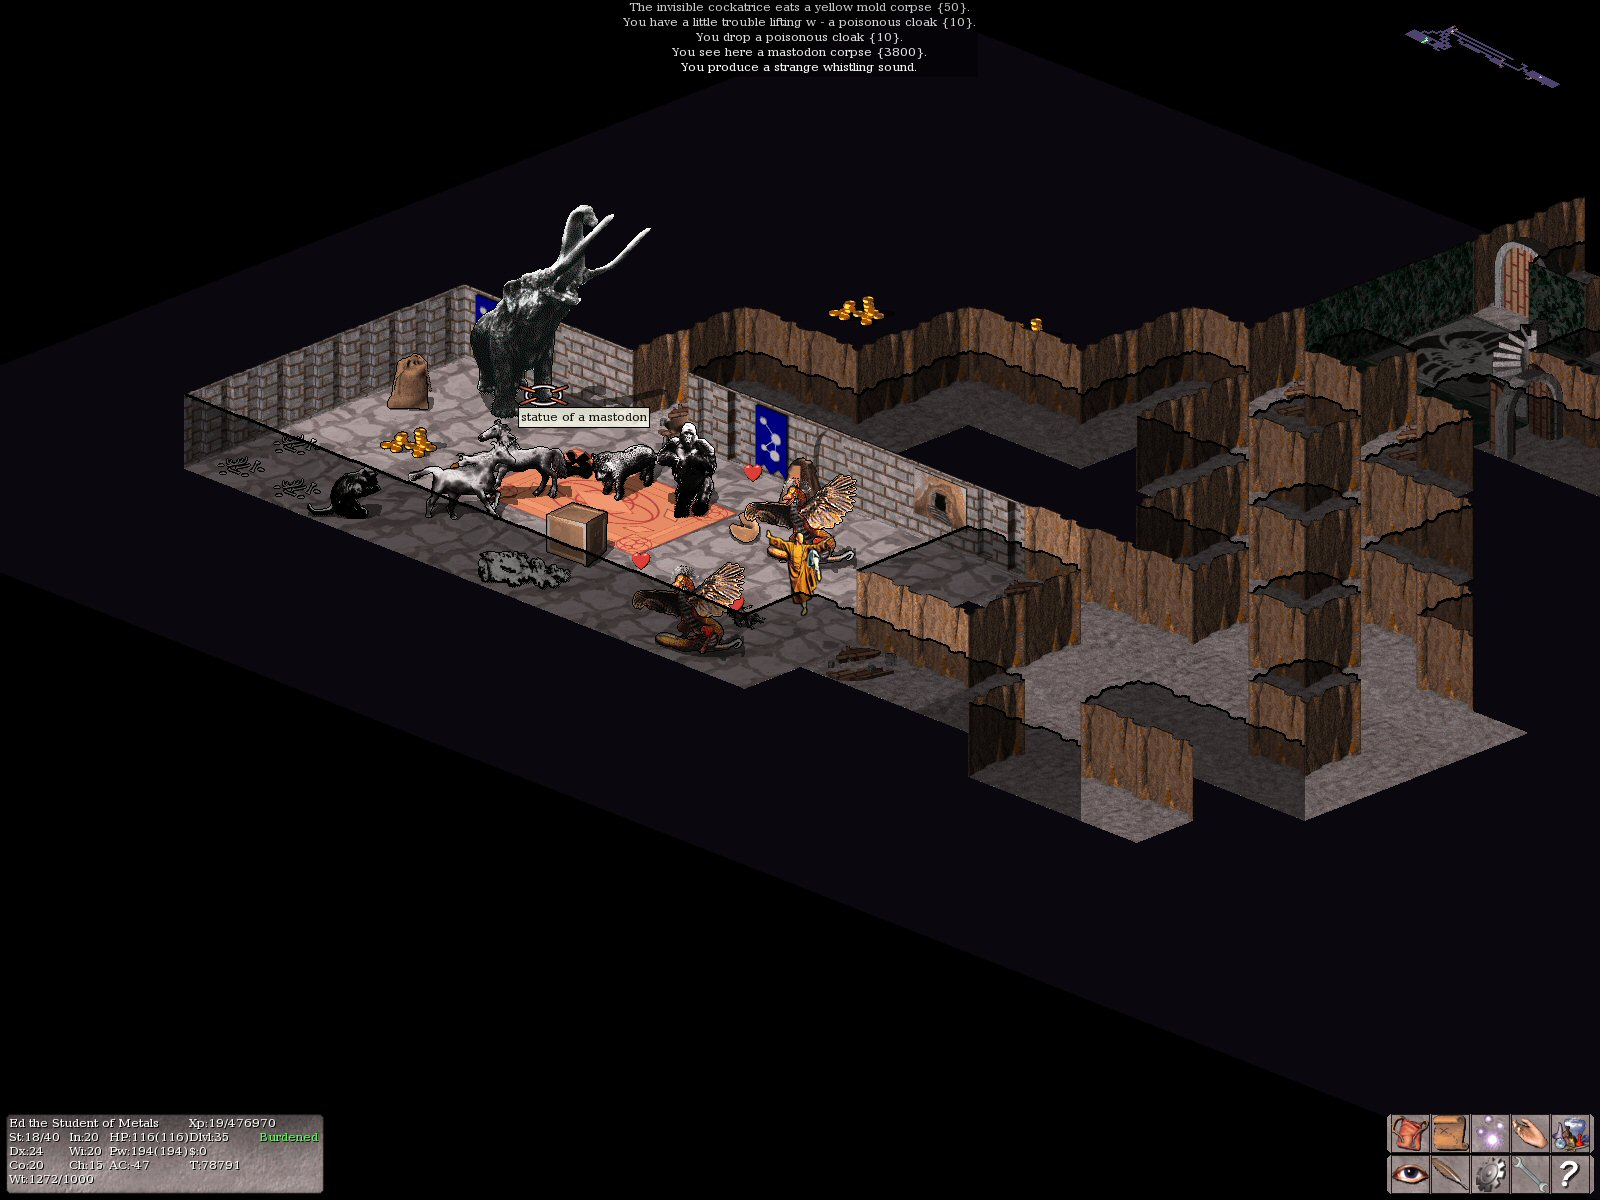
\includegraphics[width=\textwidth,height=\textheight,keepaspectratio]{./img/Vultures.jpg}
	\caption{Captura de pantalla del videojuego Vultures}
	\label{fig:vulturesgame}
\end{figure}

\subsubsection{La creación de subgéneros}

Dado que perder todo el progreso y tener que empezar desde el principio sin haber conseguido nada más que la experiencia personal es algo que no atrae a mucha gente hoy en día, son numerosos los juegos que han añadido más elementos de progreso general para que el jugador no se sienta frustrado. Estos elementos pueden ser nuevos personajes con los que jugar, puntos de experiencia o dinero con lo que poder equipar y mejorar desde un principio a nuestro personaje para poder llegar más lejos que la anterior vez, diferentes modos de juegos que se desbloquean al llegar a una cierta puntuación, etc.
También es común ver juegos que se basan en partidas cortas, de como mucho una hora, para que la repetición sea mayor y perder el personaje no sea un gran ``castigo'' que tener que afrontar.

Estos cambios que se han realizado durante los últimos años y que, de cierta manera, han modificado el género que Rogue creó en un inicio, no siempre se han tomado positivamente por parte de la comunidad, que se suele quejar de que muchos títulos que se definen a sí mismos como \textit{roguelike} no contienen ciertas características, como la dificultad, que una vez definieron el género. Por este motivo se han definido subgéneros como el \textit{roguelite}, que toman muchas de esas ideas iniciales, pero añaden o ignoran otras muchas para crear un título que sea un poco más sencillo y no penalice tanto al jugador.

\subsection{Elementos \textit{roguelike} en nuestro proyecto}

En nuestro caso hemos creado un \textit{roguelike} similar a Rogue, no solamente estéticamente, pero también en diseño y funcionalidad. El usuario se moverá por un mapa aleatoriamente generado y luchará contra diferentes enemigos que intentarán eliminarlo de diferentes formas. En base al nivel que el usuario tenga los enemigos serán más o menos complicados de batir y la recompensa por hacerlo será mayor.

El objectivo del juego es llegar lo más lejos posible dentro de la mazmorra. Cada vez que el jugador entra en un portal se añadirá un punto (el número de puntos se mostrará en la pantalla) y, cada vez que esto suceda, un nuevo mapa, con diferentes características y contenido, será generado. El juego es complicado, aleatorio y con una sensación de progreso, tal y como el género \textit{roguelike} especifica.

\begin{figure}[H]
		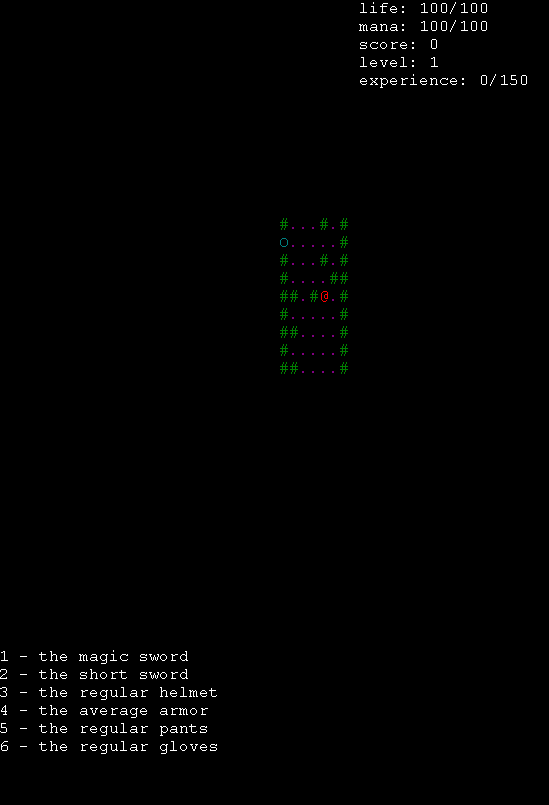
\includegraphics[width=140mm, height=185mm]{./img/roomsGameGeneral.png}
	\caption{Captura de pantalla de la interfaz de usuario de nuestro juego}
	\label{fig:roomsgamegeneral}
\end{figure}

\section{Problemas de la tecnología para ciertos sectores de la sociedad}
\label{sec:dificultadesfeedback}

Algunas de las razones que hacen de la tecnología un elemento prácticamente necesario hoy en día y que facilita su usabilidad crea, paradójicamente, una barrera para mucha gente que no puede disfrutar de ella.

En esta sección hablaremos sobre algunos de los problemas que tantos invidentes como daltónicos se encuentran actualmente en diferentes programas y cómo, en bastantes ocasiones, solventarlos no es muy complicado, lo que clarifica que muchas de estas limitaciones son dadas más por el desconocimiento que por la dificultad de la implentación de una solución.

\subsection{Dificultades a los que se enfrentan los invidentes}

Las dificultades que tienen invidentes o personas con diferentes grados de ceguera en nuestra sociedad es enorme y, tristemente, los dispositivos tecnológicos y software no se ven excluidos de esta lista. 
No poder hacer uso de una interfaz gráfica o ver lo que está sucediendo en la pantalla es un problema que automáticamente imposibiliza el uso de la mayoría de las aplicaciones y videojuegos en su totalidad. Incluso navegar por internet, donde la mayoría del contenido es texto que puede ser leído fácilmente por un lector de pantalla, puede llegar a ser un quebradero de cabeza si cierta parte de ese contenido está en flash (el lector no podrá hacer nada en este caso), los enlaces a redes sociales están en posiciones poco recomendables (dado que su contenido se puede llegar a reproducir y generalmente son un suplicio saltarlos), algunos de los nombres usados en programas software son poco descriptivos y dificultan su correcta identificación, etc.

\subsection{Cómo solventar parte de estos problemas para los invidentes}

Uno de las primeros problemas que nos comentaron en la charla de la ONCE es que muchos de los desarrolladores que programan algo específicamente para ciegos no tienen en cuenta que, la mayoría de las veces, hay gente que puede ver a su alrededor que les puede describir lo que está sucediendo en la pantalla, por lo que es muy importante crear una interfaz que esté actualizada y muestre la misma información que la persona invidente reciba.
También es necesario dar la posibilidad al usuario de repetir el contenido generado, dado que algunos lectores tienen problemas para leer ciertos caracteres o lo que leen no es del todo claro y, por lo tanto, debe de ser fácilmente repetido.

Algunos videojuegos han visto versiones adaptadas para invidentes, la mayoría de ellas desarrolladas por la comunidad, o nuevos títulos que se centran en ofrecer una experiencia revolucionaria desde el principio. Un buen ejemplo de ello es Shades of Doom\footnote{\url{http://www.gmagames.com/sod.html}}, que solamente usa sonido (principalmente ruidos repetitivos) y muy pocas frases para que el jugador sea capaz de descubrir lo que tiene que hacer y dónde está.

\subsection{Cómo hemos solventado el problema en nuestro proyecto}

En el proyecto, dado que se basa en la generación pseudo-aleatoria de frases, hemos creado descripciones para todos los elementos de la pantalla, por lo que el jugador siempre puede saber dónde se encuentra, qué hay a su alrededor, cuáles son sus características, etc. Hemos creado una ventana que se encuentra al lado del juego y donde se van guardando todas las frases generadas, siendo la primera frase la última generada y leyéndose automáticamente por el reproductor de pantalla que esté siendo usado en ese momento. De esta forma, una persona con visión siempre puede leer dicha frase y el jugador repetirla las veces que quiera.

\begin{figure}[H]
		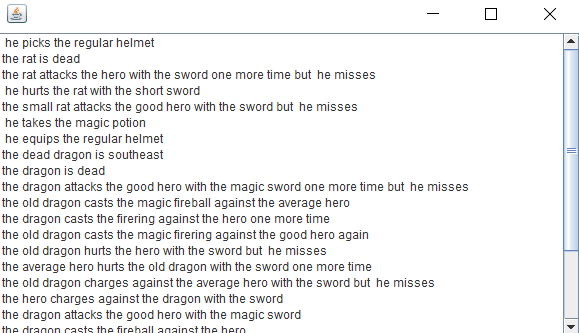
\includegraphics[width=\textwidth,height=\textheight,keepaspectratio]{./img/roomsGameTextArea.png}
	\caption{Captura de pantalla del area donde mostramos las frases generadas de nuestro juego para los invidentes}
	\label{fig:roomsgametextarea}
\end{figure}

\subsection{Dificultades a los que se enfrentan los daltónicos}

Daltonismo es un defecto genérico que afecta, aproximadamente, al 1\% de la población. Lo que en un principio parece como un pequeño inconveniente que no cambia mucho la vida de la persona que lo sufre, lo cierto es que hay muchas ocasiones en las que incluso ver un simple partido de fútbol americano correctamente puede convertirse en algo casi imposible para ellos \footnote{En \href{http://goo.gl/o3GkrP}{algunos partidos} los jugadores llevan camisetas con colores problemáticos.}. Incluso ver un mero mapa puede ser una complicación\footnote{\href{https://i.imgur.com/CMCywUU.jpg}{Resumen de algunos problemas que tienen los daltónicos a ver mapas}}.

En el mercado del ocio digital, donde los gráficos y paletas de colores juegan un gran papel en el arte del título, este problema se ve acentuado. La peor parte viene si parte de las mecánicas del juego necesitan que el jugador sea capaz de distinguir colores para obtener cierta información relevante; y esto es algo que sucede en numerosos títulos. En algunos casos es una pequeña molestia como en \textit{Borderlands}\footnote{Juego de acción en primera persona lanzado inicialmente en 2009 y que cuenta con varias secuelas} donde hay armas especiales que se diferencian, únicamente, por el color en el que se encuentra un determinado texto. Sin embargo, el mayor problema viene cuando estas limitaciones pueden llegar a arruinar el juego, como ocurre en \textit{The Witness}, un juego de puzzles mencionado en apartados anteriores en el que, para poder solventar muchos de dichos puzzles, requiere que el usuario distinga (o al menos tenga la información), distintos colores. 
También nos encontramos con juegos de lucha en dos dimensiones donde la única diferencia entre los escenarios del fondo y los personajes principales es el color de los mismos. No ver la diferencia complica a que el jugador detecte si un elemento está al frente o al fondo de dicho escenario.

\subsection{Cómo solventar parte de estos problemas para los daltónicos}
\label{sec:daltonicossolventar}

Para poder dar respuesta a esta cuestión, decidí preguntar en \textit{Reddit} a los usuarios daltónicos sobre cómo desarrollar un juego que sea adecuado para ellos \footnote{\url{https://goo.gl/d6cTqe}}. Fueron muchas las respuestas obtenidas, pero todo se puede resumir en un par de ideas.

La primera es que, en la medida de lo posible, nunca tengamos que diferenciar dos cosas distintas simplemente por el color. Tal y como un usuario comentó, si estamos desarrollando un juego naval y la diferencia entre un barco que está ``sano'' y uno que está ``roto'' es que cambiamos el color o la silueta del barco de verde a rojo, también podemos añadir chispas u otros elementos a mayores que faciliten la idea de que algo ha cambiado y ayude al usuario a apreciarlo visualmente con elementos a mayores. Del mismo modo, si tenemos un juego como \textit{Tetris} o \textit{Candy Crush} donde las piezas son relevantes, en vez de distinguirlas por color, podríamos hacerlas de diferentes formas o añadir una imagen a cada una de ellas.

La segunda idea es que, si es completamente necesario introducir diferentes colores para diferenciar ciertos elementos, o bien usamos colores que, generalmente, no crean ningún problema como el azul, amarillo, verde... (lo cual no nos garantiza que hayamos solventado el problema, dado que hay muchas formas de daltonismo y en algunas de ellas el usuario todavía puede tener problema diferenciándolos dependiendo del color contreto usado) o creamos una opción en el que podamos cambiar la paleta de colores usada. Hay algunos videojuegos (la mayor parte de ellos independientes), donde se da esta opción. 

\begin{figure}[H]
		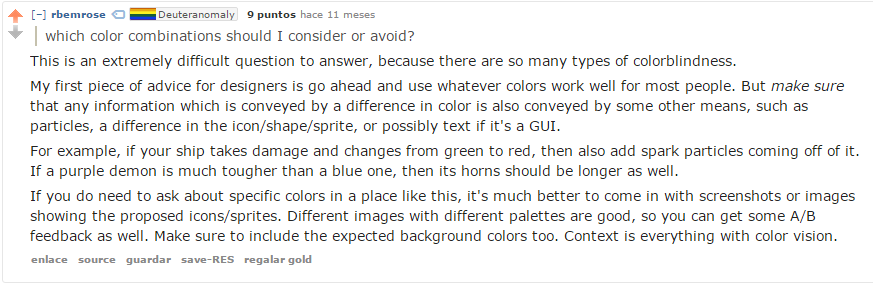
\includegraphics[width=\textwidth,height=\textheight,keepaspectratio]{./img/redditcolorblind1.png}
	\caption{Consejo para ayudar a los daltónicos a la hora de desarrollar un juego}
	\label{fig:roomsgamecolorblind1}
\end{figure}

\begin{figure}[H]
		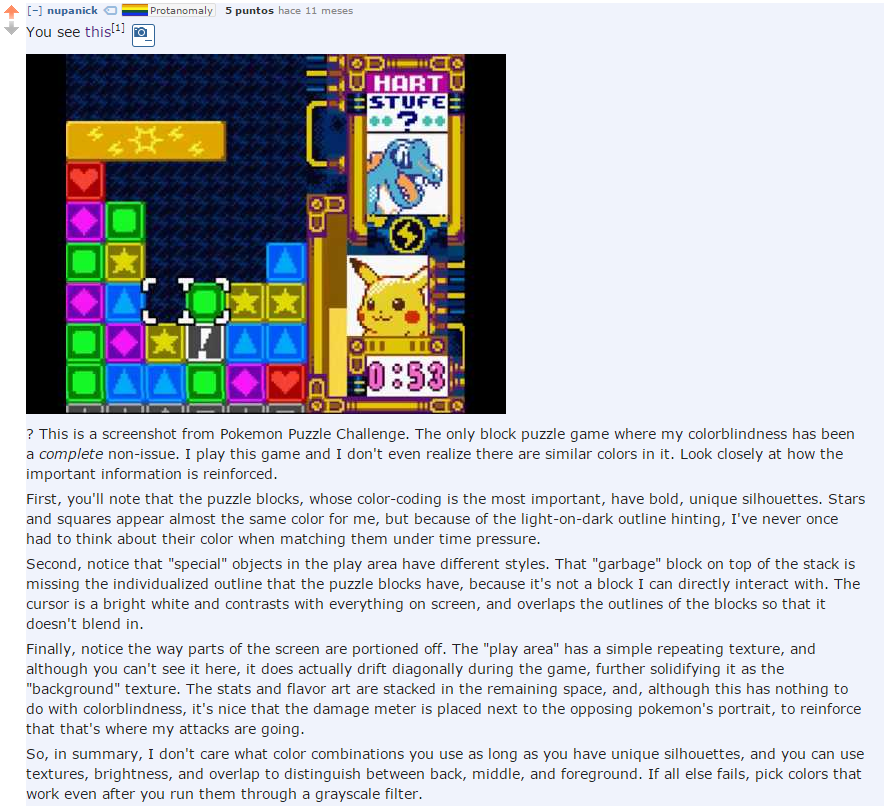
\includegraphics[width=\textwidth,height=\textheight,keepaspectratio]{./img/redditcolorblind2.png}
	\caption{Consejos y ejemplos para evitar que las personas daltónicas tengan problemas}
	\label{fig:roomsgamecolorblind2}
\end{figure}

\begin{figure}[H]
		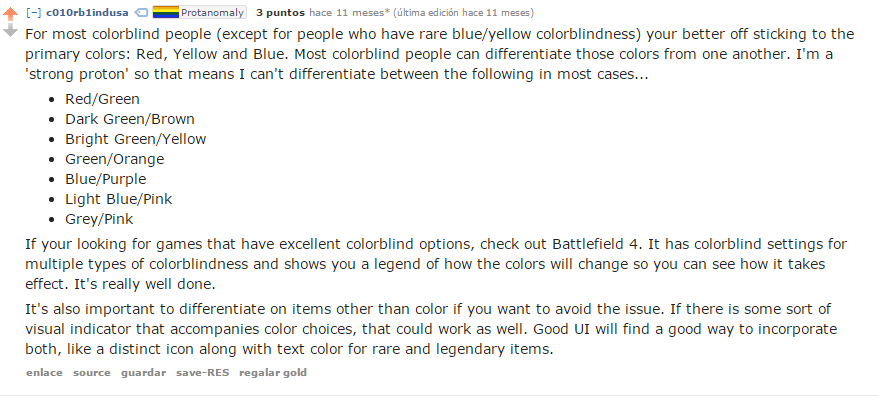
\includegraphics[width=\textwidth,height=\textheight,keepaspectratio]{./img/redditcolorblind3.png}
	\caption{Un usuario nos comenta la combinación de colores que son problemáticas}
	\label{fig:roomsgamecolorblind3}
\end{figure}

\subsection{Cómo hemos solventado el problema en nuestro proyecto}
\label{sec:solventadodaltonicos}

En nuestro caso, al haber preguntado de antemano a los usuarios, siempre tuvimos desde el primer momento la idea de crear la interfaz gráfica con soporte para daltónicos en mente, a pesar de que, al haber tenido en cuenta a las personas invidentes, cualquier persona podría jugarlo sin ninguna dificultad.

Todos los elementos que se encuentran en la pantalla están diferenciados con caracteres completamente diferentes por lo que, incluso aunque todos los colores fueran iguales, sería sencillo identificar cada elemento. 

También hemos creado una opción que cambia la paleta de colores a utilizar y facilita su visualización para aquellos usuarios con este inconveniente.

